\chapter{An advanced application: situated natural language processing}
\label{chapter|dialogs}

%%%%%%%%%%%%%%%%%%%%%%%%%%%%%%%%%%%%%%
\section{The natural language grounding process}
\label{dialog}

Verbal interaction with human presents two categories of challenges: syntactic
ones, and semantic ones. The robot must be able to process and analyze the
structure of human utterances, \ie natural language sentences, and then make
sense of them. As stated in the introduction, we process three categories of
sentences: \emph{statements}, \emph{desires} and \emph{questions} that can be
answered from the declarative knowledge present in the robot knowledge base (a
choice similar to the \emph{Behaviour Cycle} in the GLAIR
architecture~\cite{Shapiro2009}). In our work, the grounding process of the
human discourse consists in extracting either the \emph{informational} content
of the sentence to produce statements or its \emph{intentional} content (\ie
performative value) to collect orders and questions. We do not claim any
contribution to the field of computational linguists (see \cite{Kruijff2010}
for a survey of formal approaches to natural language processing in the
robotics field). Our main contribution here is the grounding (we call it
\emph{resolution}) of concepts involved in the human discourse through the
robot's own knowledge.

To this end we have developed a dedicated module called {\sc Dialogs} that processes human
input in natural language, grounds the concepts in the robot's knowledge and
eventually translates the discourse in a set of queries or declarative OWL/RDF
statements.

\begin{figure}%[!ht]
\centering
  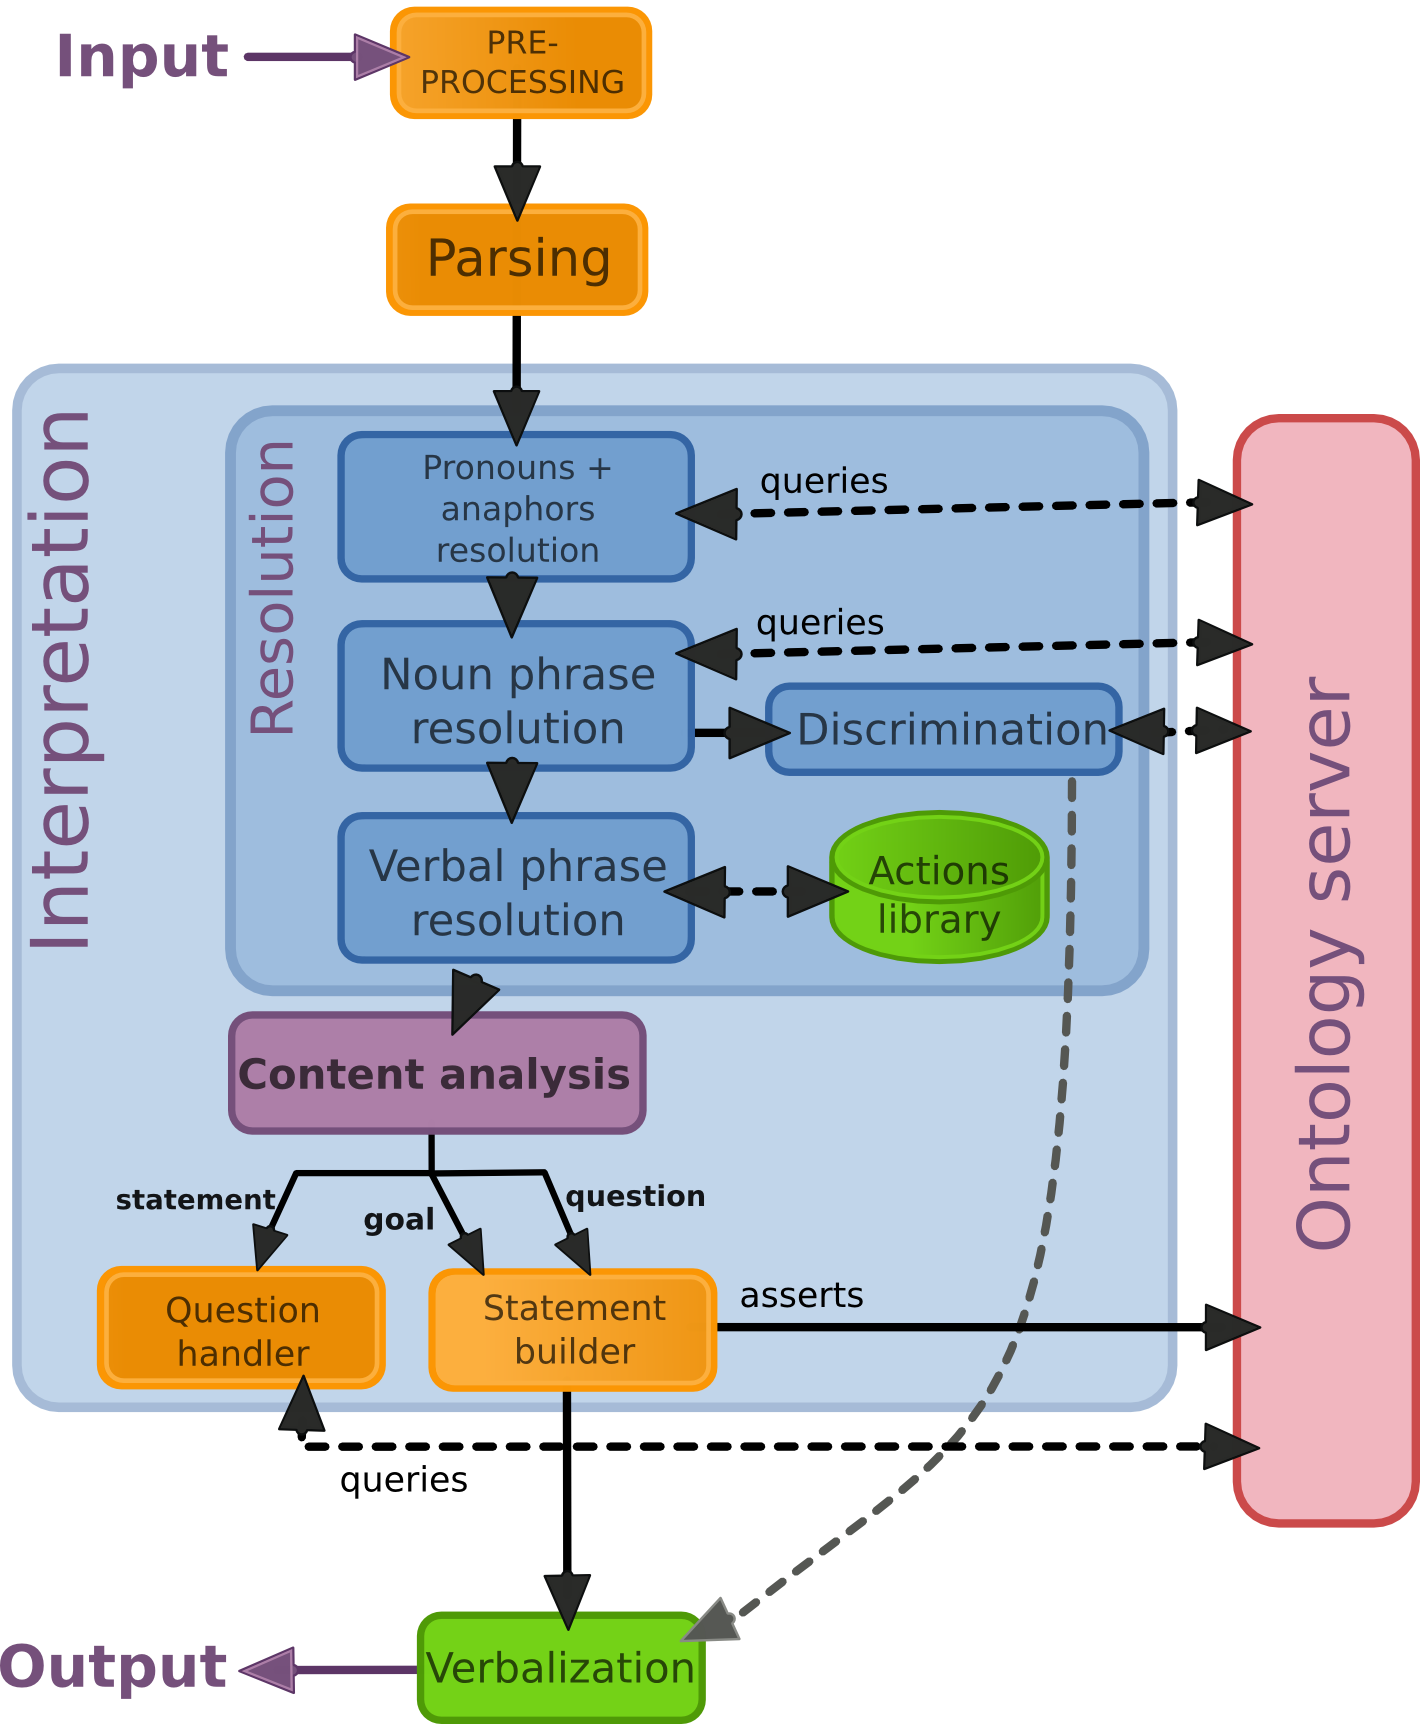
\includegraphics[width=0.9\linewidth]{dialogs/dialog_module_simple.pdf}
  \caption{The {\sc Dialogs} module has three main steps: the parsing,
  the interpretation and the verbalization. The interpretation module is
  responsible for both the \emph{resolution} and the semantic content
  \emph{analysis and translation}.} 
  \label{fig|dialog}
\end{figure}

Figure~\ref{fig|dialog} shows the {\sc Dialogs} module architecture. The user's
input is first pre-processed. For instance, \emph{I'm} constructs are expanded
into \emph{I am} and then parsed. The parser is a custom-made, rule-based (\ie
grammar-free) tool that extracts the grammatical structure from the user's
sentence. Figure~\ref{dialog|parser_output} shows an example of the raw output of the parser for a moderately complex sentence.

\begin{figure}%[!ht]
\begin{center}
\scriptsize
\begin{alltt}
>> IMPERATIVE
VP: \textbf{remember} (present simple)
    SUBSENTENCE (aim: that)
      NP: \textbf{I}
      VP: \textbf{want} (present simple)
        direct objects: 
          NP: \textbf{you}
        secondary VP: \textbf{give} ()
              direct objects:
                NP: my \emph{nice blue} \textbf{bottle}
              indirect objects:
                NP: \textbf{me}
\end{alltt}
\end{center}
\caption{Raw output of the {\sc Dialogs} parser after processing the
sentence: ``remember that I want you to give me my nice blue bottle.'' 
Nominal groups are not grounded yet.} 
\label{dialog|parser_output}
\end{figure}

The output of the parser is then sent to the \emph{interpretation} module, the
core of the component.  Interpretation consists in three distinct operations:
the sentence \emph{resolution} (concepts grounding), the \emph{content
analysis} (what is the intent of the utterance: information, question or
desire) and the \emph{statement building} (translation into RDF statements).

The sentence resolution has three steps: {\it(i)} pronouns and anaphora are
replaced by the correct speaker ID and the ID of the last object referred to
(extracted from the dialogue history) respectively, {\it(ii)} nominal groups are
disambiguated and grounded (noun phrase resolution), and {\it(iii)}
verbal groups are resolved and their associated \emph{thematic roles} are
retrieved (verbal phrase resolution).

\small
\begin{pseudocode}[ruled]{Resolution}{sentence, currentSpeaker}
\label{algo|Resolution}

\mathcal{G} \GETS \CALL{ParseNominalGroups}{sentence} \\

\FOREACH g \in \mathcal{G} \DO 
\BEGIN
   \mathcal{D} \GETS \CALL{GenerateDescription}{g} \STMTNUM{5.1em}{res.desc}\\
   candidates \GETS \CALL{Ontology.Find}{\mathcal{D}} \STMTNUM{4em}{res.onto}\\
   
   \IF \left|{candidates}\right| = 0 \THEN
    \BEGIN
      \OUTPUT{\mbox{Couldn't resolve the group!}} \\
      \EXIT \\
    \END
   \ELSEIF \left|{candidates}\right| = 1 \THEN
      id \GETS candidates[0]\\

   \ELSE
      \BEGIN
	\IF \CALL{Ontology.CheckEquivalent}{candidates} \THEN
	  id \GETS candidates[0] \\
	\ELSE
	  id \GETS \CALL{Discrimination}{candidates} \STMTNUM{0em}{st.discrimination}\\
      \END \\
   \CALL{Replace}{g, id, sentence}
\END
\end{pseudocode}
\normalsize

As represented in Figure~\ref{fig|dialog}, interpretation tightly relies on the
communication with the knowledge base. All the concepts the robot manipulates
are stored in the ontology server and retrieved through logical
queries, except for the verbs that are currently stored in a dedicated library
(the \emph{action library} in the diagram).

%%%%%%%%%%%%%%%%%%%%%%%%%%%%%%%%%%%%%
%\section{Technical analysis}
%\label{examples}


In order to better understand the overall process of the {\sc Dialogs} module 
and its relation with ORO, we next describe the different steps of the approach 
based on three examples. In these examples we assume that some initial facts 
are present in the knowledge base, both in the robot's own model and in the 
human's model.  Since the robot tries to ground a
human utterance, all queries are sent to the human model in order to interpret
it from the human perspective. 

\subsection{Informational content extraction}

\begin{figure}
    \centering
	\begin{tabular}{p{7cm}}
	\emph{Initial knowledge model of} \texttt{human\_01}\\
	\hline
    	\hspace{0.3cm}\stmt{banana\_01 type Banana} \\
    	\hspace{0.3cm}\stmt{banana\_01 hasColor yellow}\\
	
	\vspace{0.5em}
	\emph{Human input}\\
	\hline
	\hspace{0.3cm}``The yellow banana is big!'' \\

	\vspace{0.5em}
	\emph{Generated partial statements}\\
	\hline
	\hspace{0.3cm}\stmt{?obj type Banana} \\
    	\hspace{0.3cm}\stmt{?obj hasColor yellow} \\
    	\hspace{0.7cm}$\Rightarrow$ \concept{?obj = banana\_01}\\

	\vspace{0.5em}
	\emph{Newly created statements}\\
	\hline
	\hspace{0.3cm}\stmt{banana\_01 hasSize big} \\
	\end{tabular}
\caption{First example of natural language grounding: the nominal group ``the
yellow banana'' is matched with the individual \concept{banana\_01}.
``$\Rightarrow$'' represents the output of the ontology server.}
\label{dialog|ex1}
\end{figure}

Figure~\ref{dialog|ex1} shows a first example of human discourse grounding and
the extraction of informational content. We assume that the robot knowledge
base only contains two initial statements in the human model. The user
asserts a new one: ``The yellow banana is big!''. 
We first want to match the nominal group \emph{The yellow banana} to an already
known concept (algorithm~\ref{algo|Resolution}), and second to translate the property \emph{is big} into a predicate ({\tt hasSize}) to state its semantics. 

To resolve the nominal group \emph{The yellow banana} a set of partial
statements that describe the concept is generated based on the grammatical
parsing of the sentence (algorithm~\ref{algo|Resolution}(\ref{res.desc})). The parsed tree of each nominal group is translated into statements based on a set of rules.
In the example, a banana (\stmt{?obj type Banana})
that is yellow (\stmt{?obj hasColor yellow})\footnote{Predicates like
\concept{hasColor} or \concept{hasSize} that bind \concept{banana\_01} to
adjectives are extracted from a predefined database of $[Predicate \rightarrow
AdjectiveCategory]$, and falls back on the generic \concept{hasFeature}
predicate if the adjective is not known.}.  Based on these partial statements a
SPARQL query is sent to the ontology server to retrieve possible instances that match
the description (algorithm~\ref{algo|Resolution}(\ref{res.onto})).

In this first simple case, the concept \concept{banana\_01} is unambiguously
matched (since there is only one possible banana) and returned. Finally, we can now add
the new information provided by the human, \ie the new statement
\stmt{banana\_01 hasSize big}, to the human model in the ontology
server.

% The translation of \emph{yellow} to \stmt{hasColor yellow} is not obvious: in
% the general case, we associate a adjective to the noun it characterizes with
% the \concept{hasFeature} predicate (for instance, \emph{The sight is beautiful}
% would translate to \stmt{sight hasFeature beautiful}). But we can also manually
% set the predicate associated to a category of adjectives: It is what has been
% done for the main colours. Another example is the size: for known size
% adjectives (big, small, etc.), the \concept{hasSize} predicate is being used.

\subsection{Intentional content through verb resolution}
The sentence in the first example is built with the state verb \emph{be} at
indicative. Let us examine a different example with an action verb at
imperative mode (an order): ``Give me the banana". The process is
described in Figure~\ref{dialog|ex2}.

\begin{figure}
    \centering
	\begin{tabular}{p{7cm}}
	\emph{Initial knowledge model of} \texttt{human\_01}\\
	\hline
    	\hspace{0.3cm}\stmt{banana\_01 type Banana} \\
    	\hspace{0.3cm}\stmt{banana\_01 hasColor yellow}\\
	\end{tabular} \\

	\vspace{0.5em}

	\begin{tabular}{p{7cm}}
	\emph{Human input}\\
	\hline
    	\hspace{0.3cm}``Give me the banana.'' \\
	\end{tabular} \\

	\vspace{0.5em}

	\begin{tabular}{p{7cm}}
	\emph{Generated partial statements}\\
	\hline
    	\hspace{0.3cm}\stmt{?obj type Banana} \\
	\hspace{0.7cm}$\Rightarrow$ \concept{?obj = banana\_01}\\

	\end{tabular} \\

	\vspace{0.5em}

	\begin{tabular}{p{7cm}}
	\emph{Newly created statements}\\
	\hline
    	\hspace{0.3cm}\stmt{human\_01 desires situation\_a3f74} \\
    	\hspace{0.3cm}\stmt{situation\_a3f74 type Give} \\
    	\hspace{0.3cm}\stmt{situation\_a3f74 performedBy myself} \\
    	\hspace{0.3cm}\stmt{situation\_a3f74 actsOnObject banana\_01} \\
    	\hspace{0.3cm}\stmt{situation\_a3f74 receivedBy human\_01} \\
	\end{tabular}

\caption{Second example: processing an order.}
\label{dialog|ex2}
\end{figure}

\label{processing_of_actions}

In order to capture the intentional content of a sentence (for example, an
order) we need to retain the semantics of the verb and its complements.
\emph{Thematic roles} allow for semantically linking a verb to its complements.  
There is no general agreement amongst linguists on a comprehensive list of 
thematic roles. The amount and the granularity of roles varies a lot in 
the literature~\cite{Gutierrez2001}. We thus use a small set of them, which matches
the relations the robot can actually achieve (we discuss
possible extensions in the conclusion). For instance, in the second example,
the verb \emph{give} has three thematic roles: \concept{performedBy},
\concept{actsOnObject} and \concept{receivedBy}.

The list of actions the robot can plan for (currently \emph{take},
\emph{place}, \emph{give}, \emph{show}, \emph{hide} and \emph{move}) along with
possible synonyms (for example, \emph{to pick} is set as a synonym of \emph{to
take}) and their associated thematic roles are stored in a predefined library
of actions. For each action we identify and store: the role of the subject in
the sentence (always \concept{performedBy}); the role of the direct object
(for instance, \concept{actsOnObject}); and the role of each of the indirect
objects with their optional prepositions (for instance,
\concept{receivedBy})\footnote{Note that in example 2, ``give me the banana'',
the pronoun ``me'' appears before ``banana'', while it is an indirect
complement --- ``give it {\bf to me}''. The parser correctly handles these
cases.}. Moreover, through the ontology we check that each holder of a
role is semantically consistent. For instance, the action \emph{Give} must have a
manipulable physical item (\concept{Artifact}) as direct object. Thus, if the
concept the robot finds for the thematic role \concept{actsOnObject} cannot be
inferred to be an artifact, the robot goes back to the human saying it does not
understand.

This second example  also shows the pronouns reference resolution: ``me'' is
replaced by the id of the current speaker while ``you'' is replaced by
\concept{myself} (\concept{myself} always represents the robot itself). When
present, anaphoras (references to previous concepts like ``give me the banana, I
like {\bf it}.'') are also resolved in the same step.

Once the sentence is completely resolved and translated into a formal
representation (a human desire in this example\footnote{Orders are here
represented as human desires: the human desires a specific new situation.}), we
store it in the ontology server. The robot's decisional/executive layers can
then decide whether to execute the order or not. 

\subsection{Informational content extraction requiring clarification}
\label{dialogs:disamb}
\begin{figure}
    \centering
	\begin{tabular}{p{7cm}}
	\emph{Initial knowledge model of} \texttt{human\_01}\\
	\hline
     	\hspace{0.3cm}\stmt{banana\_01 type Banana} \\
     	\hspace{0.3cm}\stmt{banana\_01 hasColor yellow} \\
     	\hspace{0.3cm}\stmt{banana\_02 type Banana} \\
     	\hspace{0.3cm}\stmt{banana\_02 hasColor green} \\
	\end{tabular} \\

	\vspace{0.5em}

	\begin{tabular}{p{7cm}}
	\emph{Human input}\\
	\hline
     	\hspace{0.3cm}``The banana is good.'' \\
	\end{tabular} \\

	\vspace{0.5em}

	\begin{tabular}{p{7cm}}
	\emph{Generated partial statements}\\
	\hline
     	\hspace{0.3cm}\stmt{?obj type Banana} \\
	\hspace{0.7cm} $\Rightarrow$ \concept{?obj = [banana\_01, banana\_02]}
	\end{tabular} \\

	\vspace{0.5em}

	\begin{tabular}{p{7cm}}
	\emph{Discrimination process}\\
	\hline
     	\hspace{0.3cm}\concept{discriminate([banana\_01, banana\_02])} \\
	\hspace{0.7cm} $\Rightarrow$ \concept{?hasColor = [yellow, green]}
	\end{tabular} \\

	\vspace{0.5em}

	\begin{tabular}{p{7cm}}
	\emph{Robot output speech}\\
	\hline
     	\hspace{0.3cm}``The yellow one or the green one?'' \\
	\end{tabular} \\

	\vspace{0.5em}

	\begin{tabular}{p{7cm}}
	\emph{Human answer}\\
	\hline
     	\hspace{0.3cm}``The green one.'' \\
	\end{tabular} \\
    
	\vspace{0.5em}

	\begin{tabular}{p{7cm}}
	\emph{Extended human input}\\
	\hline
     	\hspace{0.3cm}``The green banana is good.'' \\
	\end{tabular} \\
	
	\vspace{0.5em}

	\begin{tabular}{p{7cm}}
	\emph{Generated partial statements}\\
	\hline
     	\hspace{0.3cm}\stmt{?obj type Banana} \\
     	\hspace{0.3cm}\stmt{?obj hasColor green} \\
	\hspace{0.7cm} $\Rightarrow$ \concept{?obj = [banana\_02]}
	\end{tabular} \\
    
	\vspace{0.5em}
	\begin{tabular}{p{7cm}}
	\emph{Newly created statements}\\
	\hline
     	\hspace{0.3cm}\stmt{banana\_02 hasFeature good} \\
	\end{tabular}

\caption{Ambiguity resolution: in this example, ``banana'' can refer to the
yellow banana (\concept{banana\_01}) or the green one (\concept{banana\_02}).
Discrimination routines handle the disambiguation process.} \label{dialog|ex3}
\end{figure}

This last example (Figure~\ref{dialog|ex3}) shows the resolution of ambiguous
concepts. In this case the user refers to ``the banana'' while two instances of 
the \concept{Banana} class exist in the ontology. The robot needs to find out
to which instance the user is actually referring to. To this end,
disambiguation routines (algorithm~\ref{algo|Resolution}(\ref{st.discrimination}), see \cite{Ros2010b} for details of the routines)
find differences between the instances (in the example, one banana is yellow
while the other one is green) and build a sentence through the
\emph{verbalization} module to ask the user a closed question that will
help clarify the ambiguity: ``Is it yellow or green?'' The user's answer is
parsed and merged with the previous sentence. The resulting, augmented,
sentence (``The green banana is good") goes again through all the
interpretation steps. This process is repeated until no ambiguities arise. 
In the example, the \concept{banana\_02} is finally returned.

%If no differences \fxfatal{should we say 'in the human model', even if 
%getDiscriminantForAgent currently doesn't work?} can be found, an open question 
%(``give me more information'') is send to the human.

Several other strategies are used in parallel to disambiguate concepts without
having to ask for more information to the human:

\begin{itemize}
	\item Which objects are currently visible to the human? If only one of
	them, then it is probably the one the user is talking about. 
	\item Did a previous interaction involved a specific object that would
	still be the subject of the current sentence?
	\item Is the user looking or pointing at a specific object?
\end{itemize}

%Two cases can alter the way the discrimination routines work:
%\begin{enumerate}
%    \item If a sentence starts with {\it Learn that...}, failures during 
%    discrimination are interpreted as new concepts, and instead of marking the 
%    nominal as not resolved, and new identifier is created and add to the knowledge base.
%    \item For questions like {\it Which color is the bottle?}, the discrimination 
%    algorithm can not use the feature {\it color} to identify to bottle. The 
%    resolution algorithm pass this kind of constraints as a parameter of the 
%    discrimination routines.
%\end{enumerate}

 
While no examples involving questions have been detailed, \emph{W-} questions
and \emph{yes/no} questions can be processed in a similar way by
\textsc{Dialogs}. For instance, a question like ``What is on the table?''
is grounded (to extract the relation \concept{isOn} and to find what \emph{table}
refers to) and transformed into the following kind of query: \concept{find ?var
[\stmt{?var isOn table1}]}.  Answers are converted back to a full sentence
by the \emph{verbalization} module, and uttered to the human.
